\documentclass[11pt,reqno,final]{amsart}

\pdfcompresslevel=0
\pdfobjcompresslevel=0

\usepackage[dvipsnames]{xcolor}% adds colors
\usepackage{amsmath, amsthm}% {amsfonts, amssymb}

% New Characters
\usepackage[latin1]{inputenc}%
\usepackage[T1]{fontenc}

\usepackage{MnSymbol}
\usepackage[normalem]{ulem}% underlining

\usepackage[theoremfont, largesc]{newpxtext} % different text,math font
\usepackage{newpxmath}

\makeatletter
\DeclareMathRadical{\sqrtsign}{symbols}{112}{largesymbols}{112}
\let\sqrt=\undefined
\DeclareRobustCommand\sqrt{\@ifnextchar[\@sqrt{\mathpalette\@x@sqrt}}
\def\@x@sqrt#1#2{%
 \setbox\z@\hbox{$\m@th#1\sqrtsign{\mkern1mu #2}$}
 \mkern3mu\box\z@}
\makeatother




% Page Typesetting
\usepackage[final]{microtype}
\usepackage{relsize}
\usepackage[margin=1in]{geometry}
\usepackage{framed}
\usepackage{tikz}

\usepackage{hyperref}
\hypersetup{
  final,
  pdftitle={Math 135 - Inverses},
  pdfauthor={Bonventre}, 
  linktoc=page,
  pagebackref,
  colorlinks=true,
  citecolor=PineGreen,
  linkcolor=PineGreen,
  linkbordercolor=PineGreen,
}


% Internal References

\usepackage[inline,shortlabels]{enumitem}

\numberwithin{equation}{section} 
\numberwithin{figure}{section}

\usepackage[nameinlink,capitalise,noabbrev]{cleveref}

\crefname{equation}{}{} % get \cref to behave as \eqref

% \theoremstyle{plain} % bold name, italic text
\newtheorem{theorem}[equation]{Theorem}%
\newtheorem*{theorem*}{Theorem}%
\newtheorem{lemma}[equation]{Lemma}%
\newtheorem{proposition}[equation]{Proposition}%
\newtheorem{corollary}[equation]{Corollary}%
\newtheorem{conjecture}[equation]{Conjecture}%
\newtheorem*{conjecture*}{Conjecture}%
\newtheorem{claim}[equation]{Claim}%
\newtheorem{question}{Question}

\theoremstyle{definition} % bold name, plain text
\newtheorem{definition}[equation]{Definition}%
\newtheorem*{definition*}{Definition}%
\newtheorem{example}[equation]{Example}%
\newtheorem*{example*}{Example}%
\newtheorem{remark}[equation]{Remark}%
\newtheorem{notation}[equation]{Notation}%
\newtheorem{convention}[equation]{Convention}%
\newtheorem{assumption}[equation]{Assumption}%
\newtheorem{exercise}[question]{Exercise}

% ---------- macros
\newcommand{\set}[1]{\left\{#1\right\}}%
\newcommand{\sets}[2]{\left\{ #1 \;|\; #2\right\}}%
\newcommand{\longto}{\longrightarrow}%
\newcommand{\into}{\hookrightarrow}%
\newcommand{\onto}{\twoheadrightarrow}%

\usepackage{harpoon}
\newcommand{\vect}[1]{\text{\overrightharp{\ensuremath{#1}}}}

\newcommand{\del}{\partial}%

\newcommand{\ki}{\chi}
\newcommand{\ksi}{\xi}
\newcommand{\Ksi}{\Xi}

% %%%%%%%%%%%%%%%%%%%%%%%%%%%%%%%%%%%%%%%%%%%%%%%%%%%%%%%%%%%%%%%%%%%%%%%%%%%%%%%%%%%%%%%%%%%%%%%%%%%%

\begin{document}

\begin{center}
        \textbf{\Large Math 135, Calculus 1, Fall 2020}\\[10pt]
        {\large 09-11: Composition and Inverses (Section 1.5)}
\end{center}

\thispagestyle{empty}

\renewcommand{\thesection}{\Alph{section}}

\section{Meet your classmates}

Share and discuss your experience (past or desired) at Holy Cross:
\begin{question}
        What classes are you taking this year, or want to take in the future?
        What clubs are you excited to check out, or have been part of?
        Why did you choose Holy Cross?
\end{question}


\section{Composition}

Given two functions $f$ and $g$, we may consider them in succession by \textbf{composing them together}.
This creates a new function:
\begin{framed}
        The \textbf{composite} of $f$ with $g$ is the new function $f \circ g$ given by
        \[
                (f \circ g)(x) = f(g(x)) = \mbox{ "$f$ of $g$ of $x$"}
        \]
\end{framed}

\begin{exercise}
        Suppose that $f(x) = \sqrt{x}$ and $g(x) = 3x+1$.
        Find $(f \circ g)(x)$ and $g(f(x))$.
        \vfill
        \vfill
        What is the domain of $(f \circ g)(x)$? How does it compare to the domain of $g$?
        \vfill
        What is the domain of $g(f(x))$? How does it compare to the domain of $f$?
        \vfill
\end{exercise}

\begin{exercise}
        Suppose that $f(x) = 5x-3$.
        % \begin{enumerate}[(a)]
        % \item Find a function $g(x)$ such that $f(g(x)) = x^2$.
        %         \vfill
        % \item
        Find a function $h(x)$ such that $h(f(x)) = x$.\\
        (Hint: switch the role of $y$ and $x$ in the rule for $f(x)$)
        \vfill
        % \end{enumerate}
\end{exercise}

\newpage

\section{Inverses}

We may try to ``reverse'' a function:
if $f(2) = 7$, is there a new function $f^{-1}$ such that $f^{-1}(7) = 2$?

\begin{exercise}
        Consider $f(x) = 2x-8$ and $g(x) = \frac{1}{2}x + 4$.
        \begin{enumerate}[(a)]
        \item We see $f(0) = -8$. What is $g(-8)$?\\
        \item We see $f(3) = -2$. What is $g(-2)$?\\
        \item What is $f(g(x))$?
                \vfill
        \item What is $g(f(x))$?
                \vfill
        \end{enumerate}
\end{exercise}

\begin{framed}
        The \textbf{inverse} of a function $f$, if it exists, is another function $f^{-1}$ such that
        \[
                f(f^{-1}(x)) = x \qquad \mbox{and} \qquad f^{-1}(f(x)) = x.
        \]
\end{framed}

\textbf{Warning:} $f^{-1}(x)$ is NOT the same as $\dfrac{1}{f(x)}$.\\

\begin{definition}
        A function $f$ is \textbf{one-to-one} on a domain $D$ if,
        for every value $c$, the equation $f(x) = c$ has \textit{at most} one solution $x$ in $D$.

        This is true exactly when the graph of the function passes the \textbf{horizontal line test}.
\end{definition}

\begin{theorem}
        The inverse function $f^{-1}(x)$ exists exactly when $f$ is one-to-one on its domain.\\
\end{theorem}

\begin{center}
        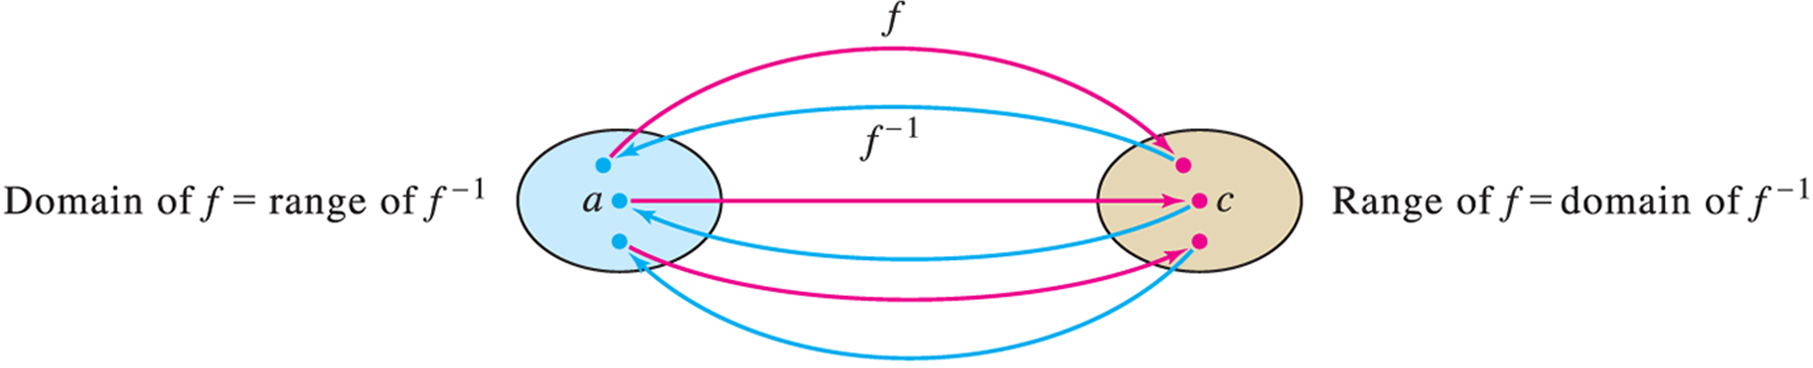
\includegraphics[width=\textwidth]{f_finv.png}
\end{center}

$ $

\begin{exercise}
        Why doesn't $f(x) = x^2$ have an inverse?
        Can we shrink the domain of $f$ so that it does?
        \vfill
\end{exercise}

\newpage



% \begin{exercise}
%         Which of the following functions has an inverse?
%         If it does, draw it on the same axes; if it doesn't, can we restrict the domain so that it does?
%         What is the domain and range of the inverse function?
%         \begin{enumerate}[(a)]
%         \item 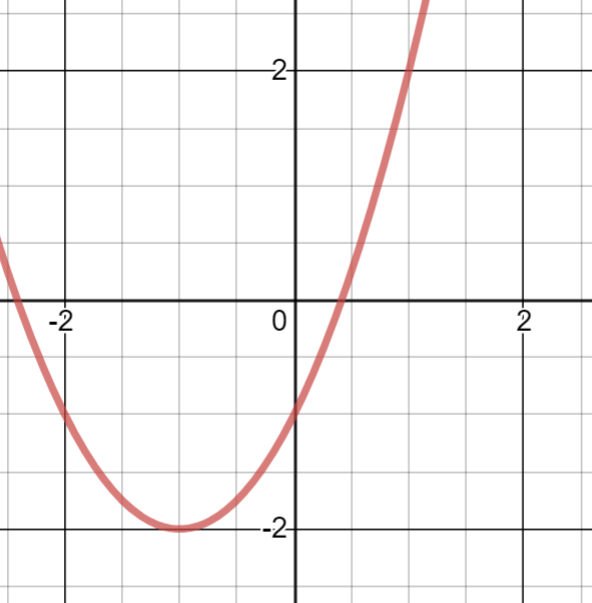
\includegraphics[width=.33\textwidth]{09-11P_1.png}
%                 \vfill
%                 \newpage
%         \item 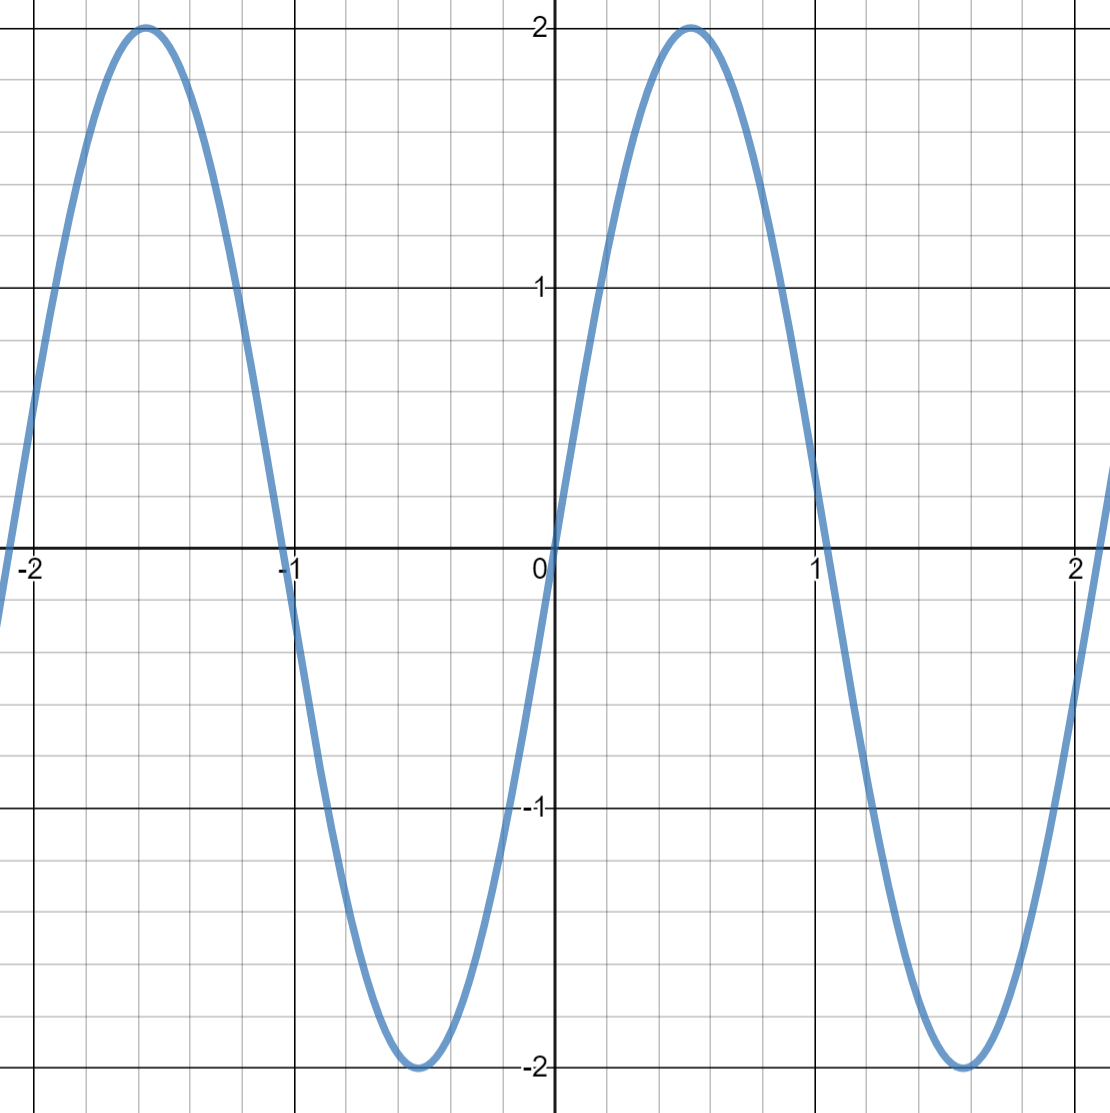
\includegraphics[width=.33\textwidth]{09-11P_2.png}\\
%         \item 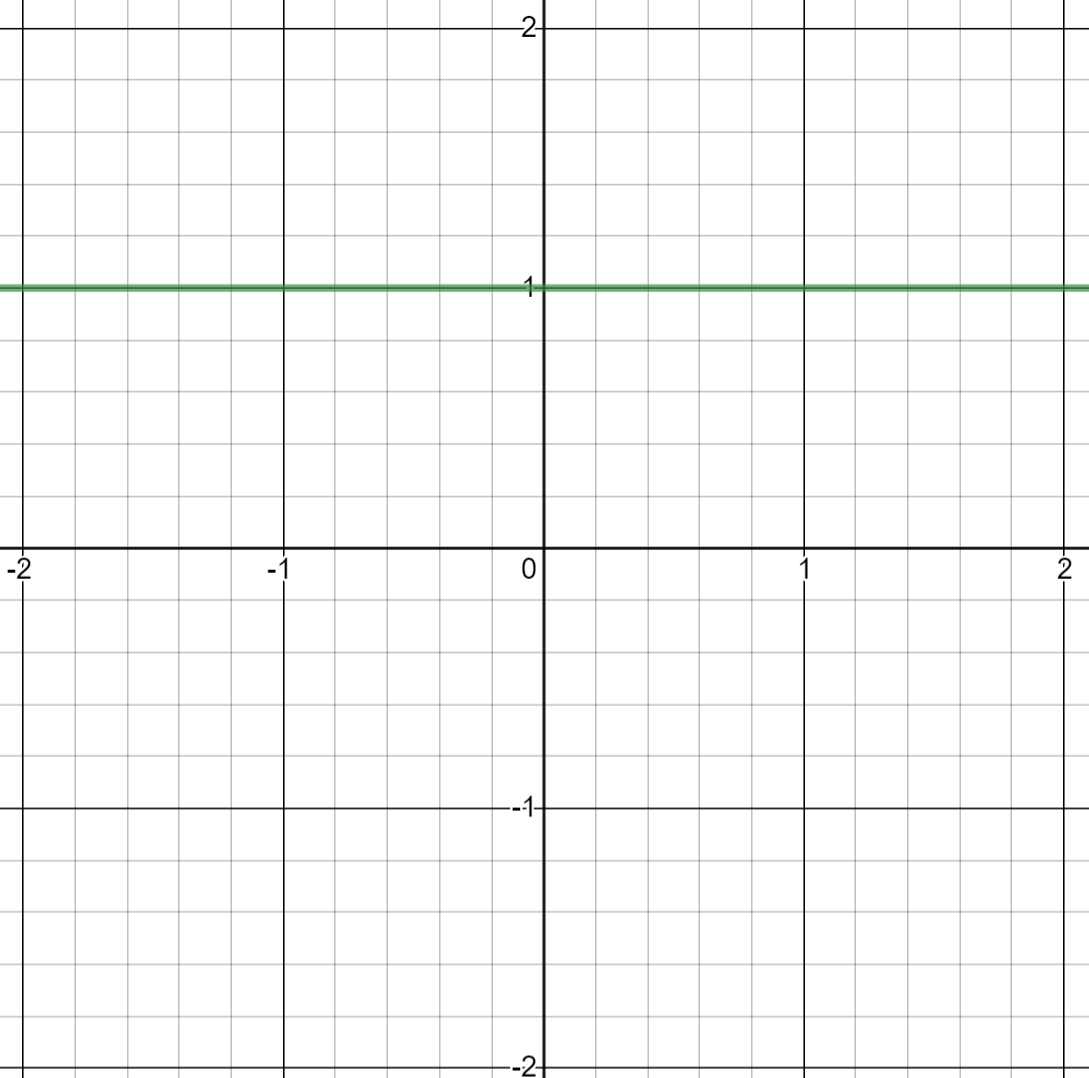
\includegraphics[width=.33\textwidth]{09-11P_3.png}
%         \end{enumerate}
% \end{exercise}

\newpage


\section{Inverse Trig Functions}

$ $

\begin{minipage}{.6\textwidth}
        \begin{center}
                % 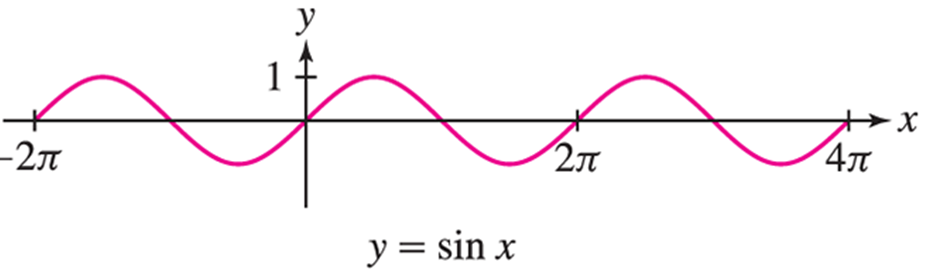
\includegraphics[width=3in]{sin.png}\\
                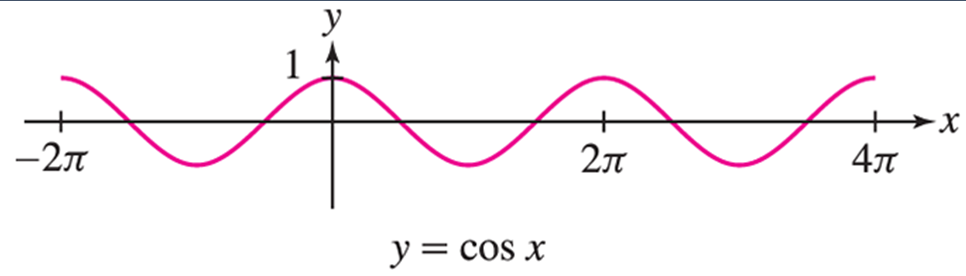
\includegraphics[width=3.3in]{cos.png}\\
                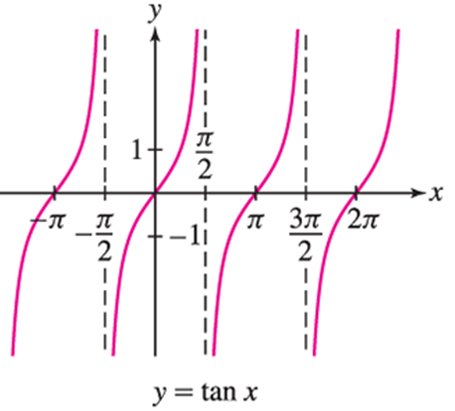
\includegraphics[width=2.2in]{tan.png}
        \end{center}
\end{minipage}
\begin{minipage}{.4\textwidth}
        \textbf{None} of the trig functions satisfy the horizontal line test.
        This means that they don't have inverses over their whole domain.
        Instead, we \textbf{restrict} the domain of each trig function so that they do.\\
        
        For example, to define the inverse of $\sin \theta$, denoted $\sin^{-1}(\theta)$ or $\arcsin \theta$,
        we restrict the domain of $\sin \theta$ to $[-\pi/2,\pi/2]$,
        where it passes the horizontal line test.
\end{minipage}

\begin{center}
        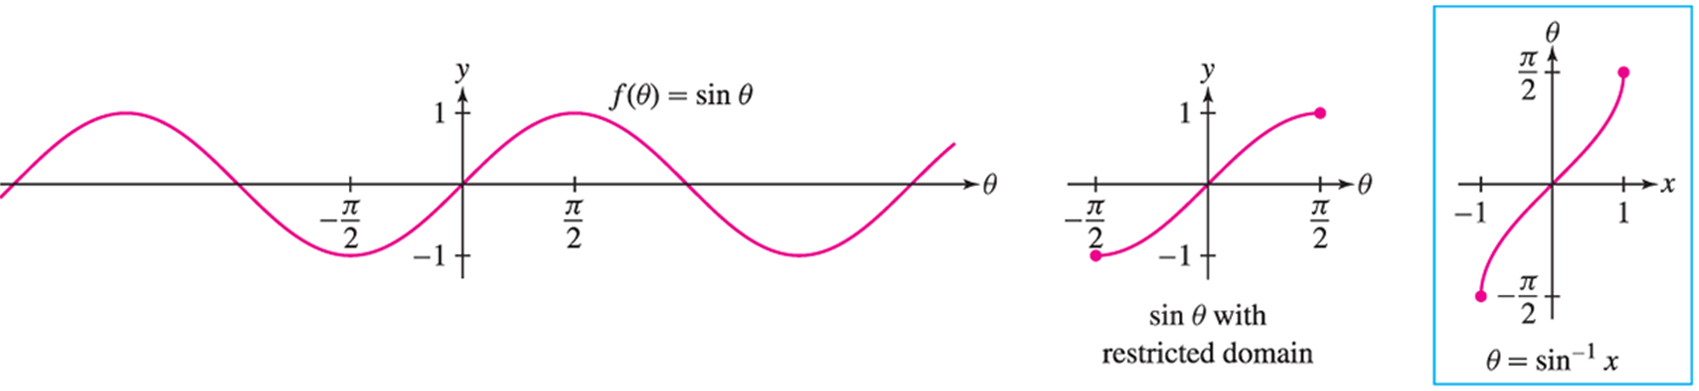
\includegraphics[width=\textwidth]{restrict_sin.png}
\end{center}



\begin{exercise}
        We have stated the restricted domain we will use for each trig function below.
        Complete the rest of the table.\\        
        {\renewcommand{\arraystretch}{3}%                
          \begin{tabular}{|c|c|c||c|c|c|}
            \hline
            function & restricted domain & \qquad range \qquad $ $ & inverse function & \qquad domain \qquad $ $ & \qquad range \qquad $ $ \\ \hline \hline
            $\cos(x)$ & $[0,\pi]$ & & $\cos^{-1}(x)$ & & \\ \hline
            $\sin(x)$ & $[-\pi/2,\pi/2]$ & & $\sin^{-1}(x)$ & & \\ \hline
            $\tan(x)$ & $(-\pi/2,\pi/2)$ & & $\tan^{-1}(x)$ & & \\ \hline
            %$\cot(x)$ & $(0,\pi)$ & & $\cot^{-1}(x)$ & & \\ \hline
            %$\sec(x)$ & $[0, \pi/2) \cup (\pi/2, \pi]$ & & $\sec^{-1}(x)$ & & \\ \hline
            %$\csc(x)$ & $[-\pi/2,0) \cup (0, \pi/2]$ & & $\csc^{-1}(x)$ & & \\ \hline
          \end{tabular}
        }
\end{exercise}

\begin{exercise}
        Find all solutions $0 \leq \theta \leq 2\pi$ to $\sin \theta = \dfrac{-1}{2}$. How does your answer compare to $\sin^{-1}\left(\dfrac{-1}{2}\right)$?
\end{exercise}

\end{document}
\newpage


\section{Exponential Functions and the Logarithm}




The inverse of the exponential function $f(x) = b^x$ is called the \textbf{logarithm with base $b$}, denoted $\log_b(x)$.
Using the definition of the inverse, we have
\begin{framed}
        \[
                y = b^x \mbox{ exactly when } \log_b(y) = x
        \]
\end{framed}

\begin{exercise}
        Use the above to compute $b^{\log_b x}$ and $\log_b(b^x)$.\\
        (Hint: \textbf{inverses!} The answer should not be complicated.)
        \vfill.
\end{exercise}

\begin{exercise}
        Compute $\log_2(8)$.
        \vfill
\end{exercise}

\textbf{Euler's number} is the irrational number $e \approx 2.718$.        
The associated exponential $e^x$ has good properties (to be discovered later).
The associated logarithm $\log_e(x) = \ln(x)$ is called the \textbf{natural logarithm}.

\begin{exercise}
        Compute the domain and range of $\ln(x)$.
        \vfill
\end{exercise}

\begin{exercise}
        Use the laws of exponents to compute the following without a calculator (all answers are integers):
        \begin{enumerate}[(a)]
        \item $\log_b(1)$ \vfill
        \item $\ln(e)$ \vfill
        \item $\log_6(9) + \log_6(4)$ \vfill
        \end{enumerate}
\end{exercise}


\end{document}




\newpage

